\documentclass{beamer}
\usepackage[utf8]{inputenc}

\usetheme{Madrid}
\usecolortheme{default}
\usepackage{amsmath,amssymb,amsfonts,amsthm}
\usepackage{txfonts}
\usepackage{tkz-euclide}
\usepackage{listings}
\usepackage{adjustbox}
\usepackage{array}
\usepackage{tabularx}
\usepackage{gvv}
\usepackage{lmodern}
\usepackage{circuitikz}
\usepackage{tikz}
\usepackage{graphicx}

\setbeamertemplate{page number in head/foot}[totalframenumber]

\usepackage{tcolorbox}
\tcbuselibrary{minted,breakable,xparse,skins}



\definecolor{bg}{gray}{0.95}
\DeclareTCBListing{mintedbox}{O{}m!O{}}{%
  breakable=true,
  listing engine=minted,
  listing only,
  minted language=#2,
  minted style=default,
  minted options={%
    linenos,
    gobble=0,
    breaklines=true,
    breakafter=,,
    fontsize=\small,
    numbersep=8pt,
    #1},
  boxsep=0pt,
  left skip=0pt,
  right skip=0pt,
  left=25pt,
  right=0pt,
  top=3pt,
  bottom=3pt,
  arc=5pt,
  leftrule=0pt,
  rightrule=0pt,
  bottomrule=2pt,

  colback=bg,
  colframe=orange!70,
  enhanced,
  overlay={%
    \begin{tcbclipinterior}
    \fill[orange!20!white] (frame.south west) rectangle ([xshift=20pt]frame.north west);
    \end{tcbclipinterior}},
  #3,
}
\lstset{
    language=C,
    basicstyle=\ttfamily\small,
    keywordstyle=\color{blue},
    stringstyle=\color{orange},
    commentstyle=\color{green!60!black},
    numbers=left,
    numberstyle=\tiny\color{gray},
    breaklines=true,
    showstringspaces=false,
}
%------------------------------------------------------------
%This block of code defines the information to appear in the
%Title page
\title %optional
{3.3.15}
\date{\today}
%\subtitle{A short story}

\author % (optional)
{Shivam Sawarkar \\ AI25BTECH11031}



\begin{document}


\frame{\titlepage}
\begin{frame}{Question}
    Find the value of $x$ such that the points $A (3, 2, 1) , B (4, x, 5) , C (4, 2, -2)$ and $D (6, 5, -1)$ are coplanar.
\end{frame}

\begin{frame}{Solution}
    Let the plane (not passing through the origin) be given by
\begin{align}
\vec{n}^\top\vec{x}=1,\qquad 
\vec{n}=\myvec{n_1 \\ n_2 \\ n_3}
\end{align}
Since the points 
\begin{align}
    \vec{A}=\myvec{3 \\ 2 \\ 1} \quad
    \vec{B}=\myvec{4 \\ 2 \\ -2} \quad
    \vec{C}=\myvec{6 \\ 5 \\ -1}
\end{align}
lie on the plane, they satisfy 
\begin{align}
    \vec{n}^\top\vec{A}=1 \\ 
    \vec{n}^\top\vec{B}=1 \\ 
    \vec{n}^\top\vec{C}=1
\end{align}
\end{frame}

\begin{frame}{Solution}
    \begin{align}
\myvec{
3 & 2 & 1\\ 
4 & 2 & -2\\ 
6 & 5 & -1
}
\myvec{n_1\\ n_2\\ n_3}
=
\myvec{1 \\ 1 \\ 1}.
\end{align}

Thus
\begin{align}
n_1=\frac{9}{16},\qquad n_2=-\frac{7}{16},\qquad n_3=\frac{3}{16}.
\end{align}

Now require B to lie on the same plane:
\begin{align}
\vec{n}^\top\vec{B}=1 \\ 
\myvec{\frac{9}{16} & \frac{-7}{16} & \frac{3}{16}}\myvec{4 \\ x \\ 5}=1
\end{align}
\begin{align}
\frac{36}{16} - \frac{7}{16}x + \frac{15}{16} = 1 \\ 
x=5
\end{align}
\end{frame}

\begin{frame}{Plot}
    \begin{figure}
        \centering
        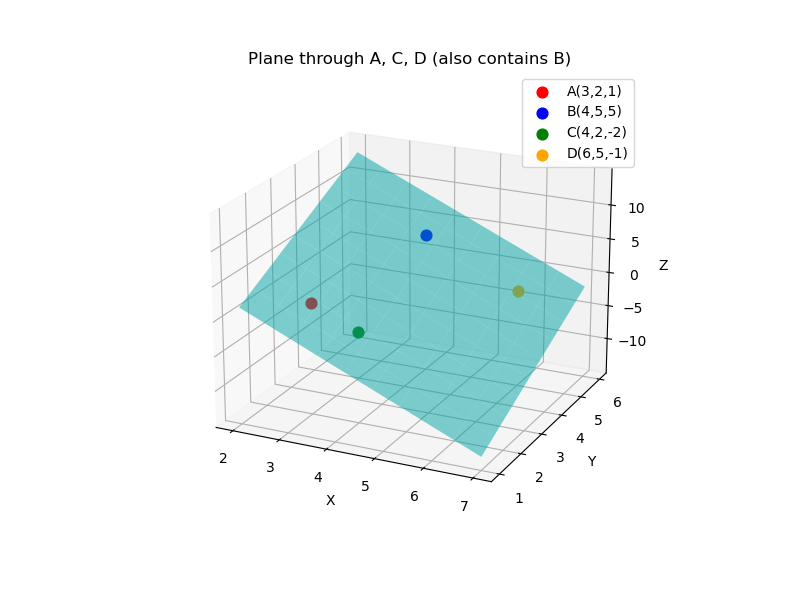
\includegraphics[width=1\linewidth]{figs/plot7.png}
        \caption{}
        \label{fig:placeholder}
    \end{figure}
\end{frame}

\begin{frame}[fragile]{C Code}
    \begin{verbatim}
#ifndef COPLANAR_H
#define COPLANAR_H

#include <stdio.h>

typedef struct {
    double x;
    double y;
    double z;
} Point;

// Function to compute vector b-a
Point vector(Point a, Point b) {
    Point res = {b.x - a.x, b.y - a.y, b.z - a.z};
    return res;
}
    \end{verbatim}
\end{frame}

\begin{frame}[fragile]{C Code}
    \begin{verbatim}
// Cross product
Point cross(Point u, Point v) {
    Point res = {
        u.y * v.z - u.z * v.y,
        u.z * v.x - u.x * v.z,
        u.x * v.y - u.y * v.x
    };
    return res;
}

// Dot product
double dot(Point u, Point v) {
    return u.x * v.x + u.y * v.y + u.z * v.z;
}
    \end{verbatim}
\end{frame}

\begin{frame}[fragile]{C Code}
    \begin{verbatim}
// Function to compute value of x for coplanarity
double solve_for_x(Point A, Point C, Point D) {
    // AC and AD vectors
    Point AC = vector(A, C);
    Point AD = vector(A, D);
    // Cross product AC × AD
    Point cross_prod = cross(AC, AD);
    // Scalar triple product condition:
    // (1, x-2, 4) ⋅ (cross_prod) = 0
    // => coeff_x * x + constant = 0
    double coeff_x = cross_prod.y;
    double constant = cross_prod.x + (-2)*cross_prod.y + 4*cross_prod.z;
    return -constant / coeff_x;
}
#endif
    \end{verbatim}
\end{frame}

\begin{frame}[fragile]{C Code}
    \begin{verbatim}
#include "solution.h"

int main() {
    Point A, C, D;
    // Input A, C, D
    printf("Enter coordinates of A (x y z): ");
    scanf("%lf %lf %lf", &A.x, &A.y, &A.z);
    printf("Enter coordinates of C (x y z): ");
    scanf("%lf %lf %lf", &C.x, &C.y, &C.z);
    printf("Enter coordinates of D (x y z): ");
    scanf("%lf %lf %lf", &D.x, &D.y, &D.z);
    // Solve for x
    double x = solve_for_x(A, C, D);
    printf("The value of x such that A, B, C, D are coplanar is: %.2f\n", x);
    return 0;
}
    \end{verbatim}
\end{frame}

\begin{frame}[fragile]{Python Code}
    \begin{verbatim}
import numpy as np

def solve_for_x(A, C, D):
    # Convert to numpy arrays
    A, C, D = np.array(A), np.array(C), np.array(D)

    # Step 1: compute vectors AC and AD
    AC = C - A
    AD = D - A

    # Step 2: normal vector n = AC × AD
    n = np.cross(AC, AD)

    # Step 3: vector (B-A) = (1, x-2, 4)
    coeff_x = n[1]
    constant = n[0]*1 + n[1]*(-2) + n[2]*4
    \end{verbatim}
\end{frame}

\begin{frame}[fragile]{Python Code}
    \begin{verbatim}
    x = -constant / coeff_x
    return x

if __name__ == "__main__":
    # Take inputs
    A = list(map(float, input("Enter coordinates of A (x y z): ").split()))
    C = list(map(float, input("Enter coordinates of C (x y z): ").split()))
    D = list(map(float, input("Enter coordinates of D (x y z): ").split()))

    x_value = solve_for_x(A, C, D)
    print("The value of x such that A, B, C, D are coplanar 
    is:", round(x_value, 2))
    \end{verbatim}
\end{frame}

\begin{frame}[fragile]{Python + C Code}
    \begin{verbatim}
import ctypes

# Load the shared library
lib = ctypes.CDLL("./solution.so")

# Define the Point struct in Python
class Point(ctypes.Structure):
    _fields_ = [("x", ctypes.c_double),
                ("y", ctypes.c_double),
                ("z", ctypes.c_double)]

# Tell ctypes about the function signature
lib.solve_for_x.argtypes = [Point, Point, Point]
lib.solve_for_x.restype = ctypes.c_double
    \end{verbatim}
\end{frame}

\begin{frame}[fragile]{Python + C Code}
    \begin{verbatim}
if __name__ == "__main__":
    A_vals = list(map(float, input("Enter coordinates of A 
    (x y z): ").split()))
    C_vals = list(map(float, input("Enter coordinates of C 
    (x y z): ").split()))
    D_vals = list(map(float, input("Enter coordinates of D 
    (x y z): ").split()))

    A = Point(*A_vals)
    C = Point(*C_vals)
    D = Point(*D_vals)

    x_value = lib.solve_for_x(A, C, D)

    print("The value of x such that A, B, C, D are coplanar 
    is:", round(x_value, 2))
    \end{verbatim}
\end{frame}




\end{document}